\begin{figure*}
    \centering
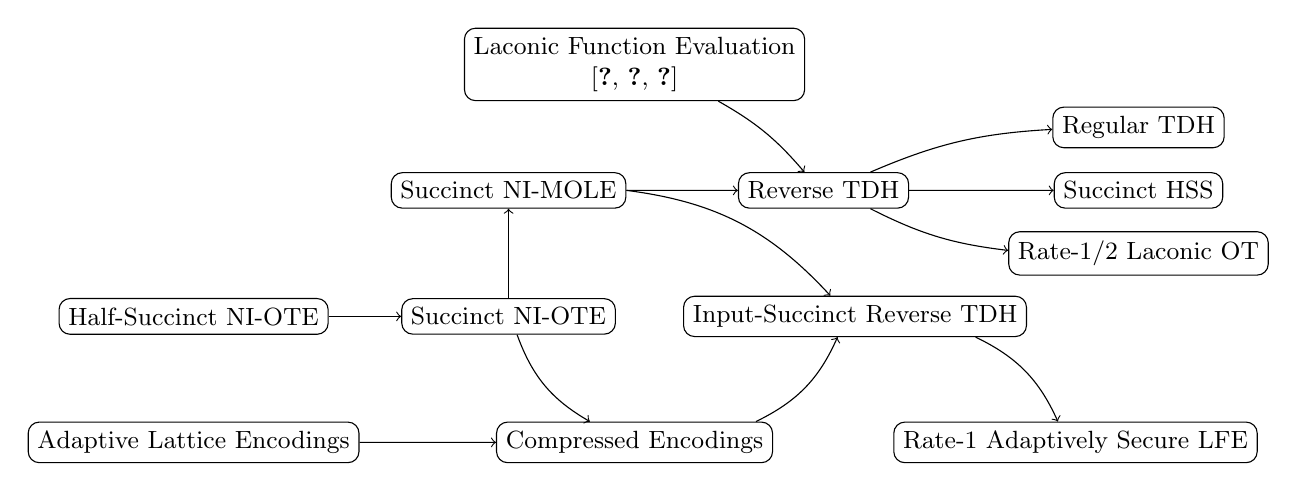
\begin{tikzpicture}[
  node distance=2cm and 3cm,
  primitive/.style={draw, rounded corners, align=center, font=\small},
  ref/.style={font=\scriptsize, midway, sloped, above},
  ref-nonsloped/.style={font=\scriptsize},
  scale = 0.8
]

% Nodes
\node[primitive] (half) at (-5,0) {Half-Succinct NI-OTE%\\(Section~\ref{sec:halfNIOTE})
};
\node[primitive] (niote) at (0,0) {Succinct NI-OTE%\\(Section~\ref{sec:NIOTE})
};
\node[primitive] (mole) at (0,2) {Succinct NI-MOLE%\\(Section~\ref{sec:MOLE})
};
\node[primitive] (lenc) at (-5,-2) {Adaptive Lattice Encodings%\\(Section~\ref{sec:hom_enc})
};
\node[primitive] (comp) at (2,-2) {Compressed Encodings%\\(Section~\ref{sec:comp_enc})
};
\node[primitive] (LFE) at (2,4) {Laconic Function Evaluation\\ \cite{FOCS:QuaWeeWic18,FOCS:HsiLinLuo23,C:DHMWW24}};
\node[primitive] (RTDH) at (5,2) {Reverse TDH%\\(Section~\ref{sec:rtdh})
};
\node[primitive] (TDH) at (10,3) {Regular TDH};
\node[primitive] (HSS) at (10,2) {Succinct HSS};
\node[primitive] (LOT) at (10,1) {Rate-$1/2$ Laconic OT};
\node[primitive] (wRTDH) at (5.5,0) {Input-Succinct Reverse TDH%\\(Section~\ref{sec:weakTDH})
};
\node[primitive] (mainLFE) at (9,-2) {Rate-1 Adaptively Secure LFE%\\(Section~\ref{sec:mainLFE})
};


% % Arrows
\draw[->] (half) -- (niote);
\draw[->] (niote) -- (mole);
\draw[->] (mole) -- (RTDH);
\draw[->] (LFE) to [bend left=10] node{} (RTDH);
\draw[->] (RTDH) to [bend left=10] node{} (TDH);
\draw[->] (RTDH) -- (HSS);
\draw[->] (RTDH) to [bend right=10] node{} (LOT);
\draw[->] (niote) to [bend right=20] node{} (comp);
\draw[->] (lenc) -- (comp);
\draw[->] (comp) to [bend right=20] node{} (wRTDH);
\draw[->] (mole) to [bend left=20] node{} (wRTDH);
\draw[->] (wRTDH) to [bend left=20] node{} (mainLFE);


\end{tikzpicture}
\caption{A schematic representation of our results, and a summary of the implications to different cryptographic primitives.}\label{fig:diagram}
\end{figure*}